\chapter{Implementacja}
\begin{figure}[h]
 \centering
 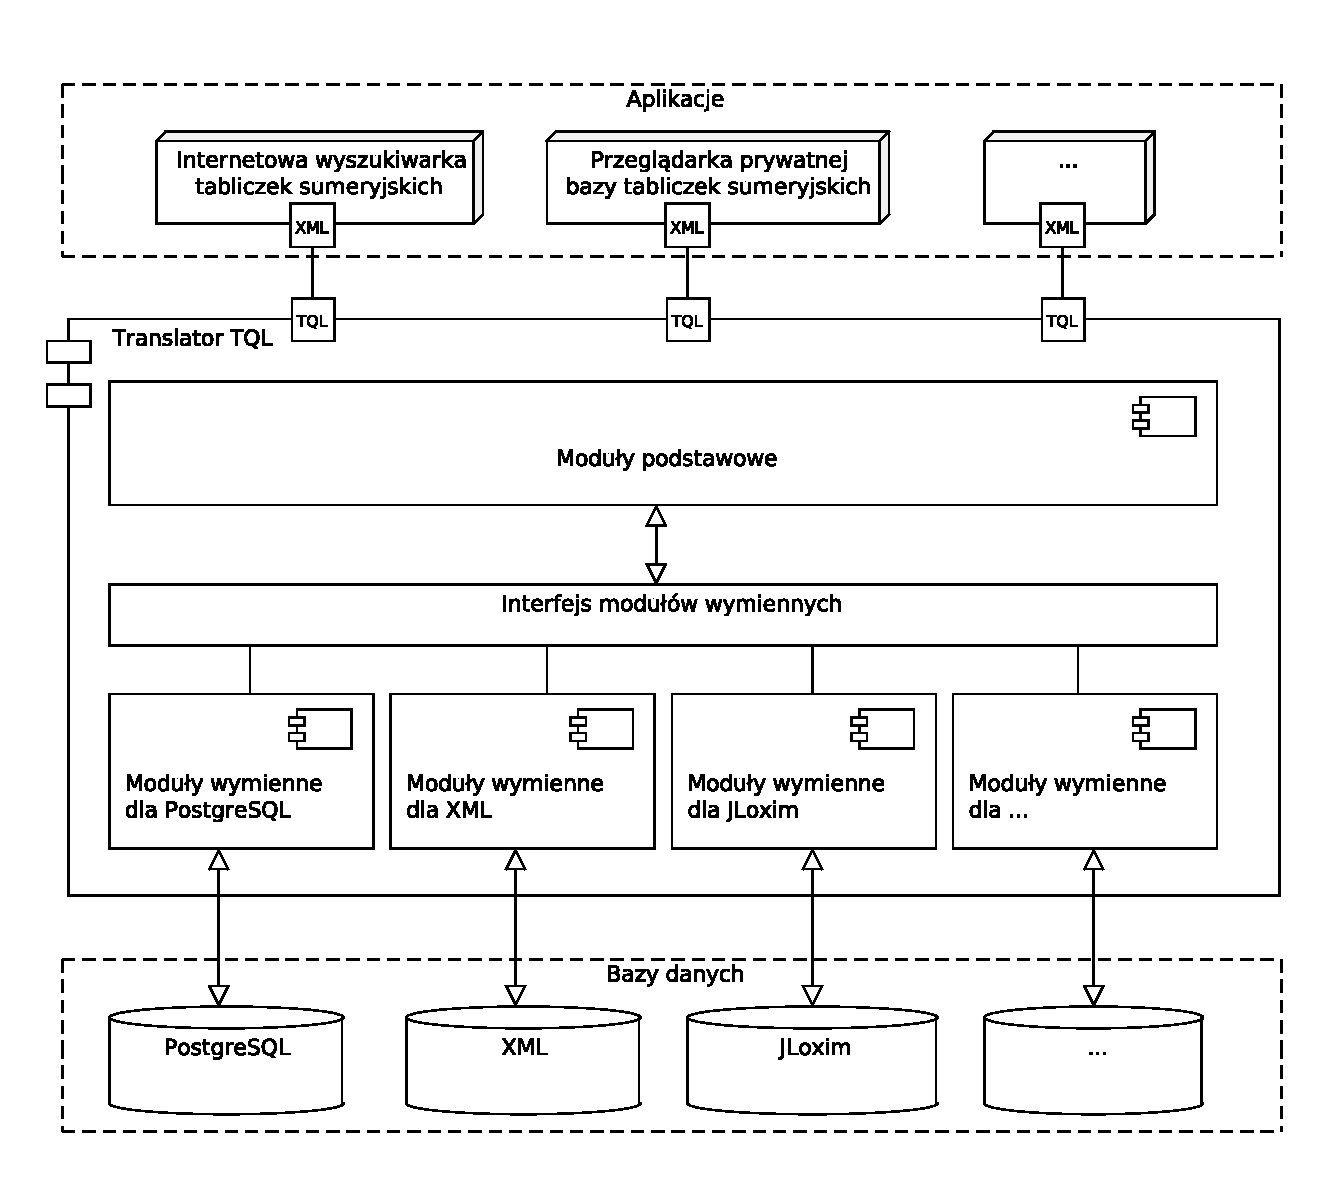
\includegraphics[width=450px,bb=0 0 608 517]{../diagramy/struktura2.pdf}
 % struktura.pdf: 608x517 pixel, 72dpi, 21.45x18.24 cm, bb=0 0 608 517
 \caption{Struktura systemu korzystającego z translatora}
\end{figure}

\begin{figure}
 \centering
 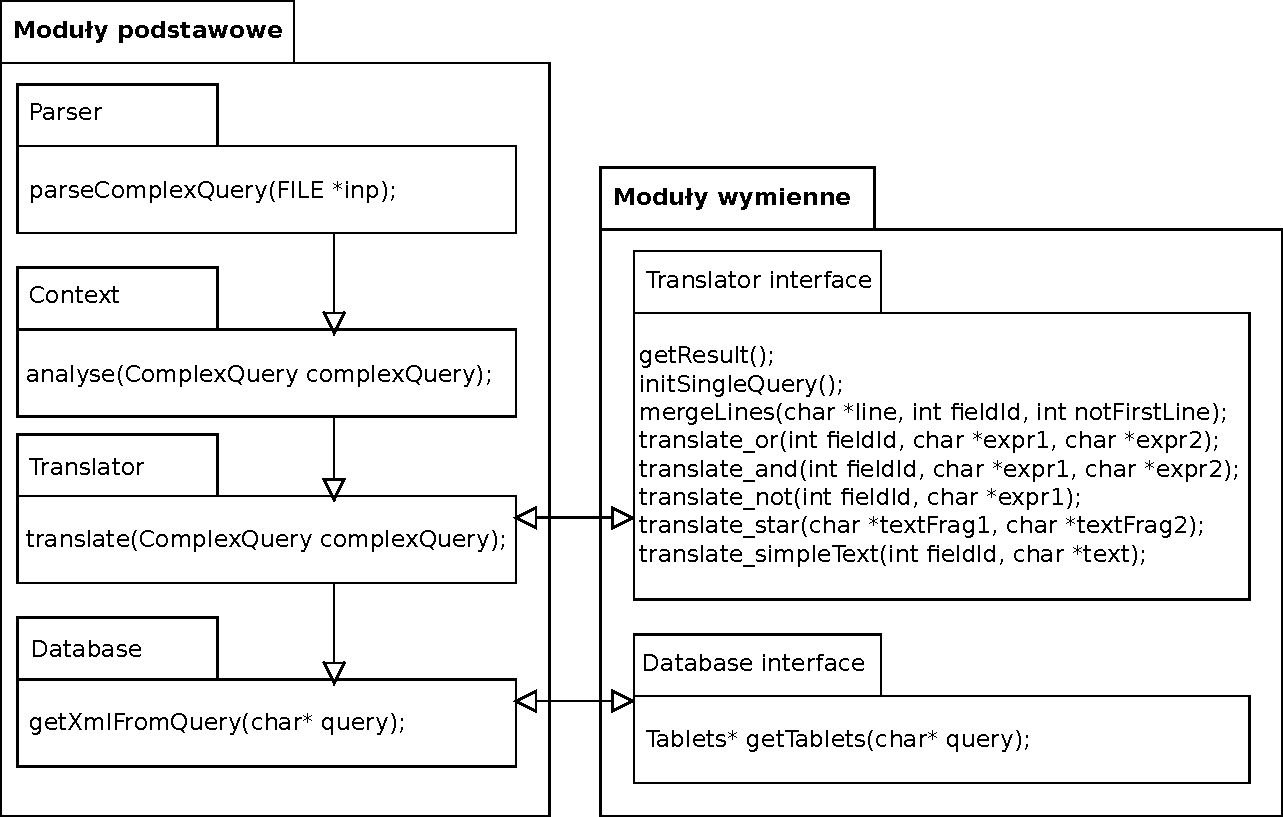
\includegraphics[width=500px]{../diagramy/pakiety.pdf}
 % pakiety.pdf: 585x300 pixel, 72dpi, 20.64x10.58 cm, bb=0 0 585 300
 \caption{Podział programu na moduły}
\end{figure}
Jednym z głównych założeń języka TQL jest niezależność od struktury danych.
W związku z tym istotną cechą translatora jest możliwość dostosowania do współpracy z różnymi bazami danych.
%Jednym z głównych wymagań postawionych przed translatorem, żeby można było podłączyć różne bazy danych.
 Wynikiem tego jest podział translatora na 2 rodzaje modułów:
\begin{enumerate}
 \item \textbf{Podstawowe} -- niezależne od struktury danych i zajmujące się głównie parsowaniem i analizą składniową zapytania.
 \item \textbf{Wymienne} -- zależne od struktury danych, tłumaczące zapytanie TQL na język odpowiedni dla używanej bazy danych
i wywołujące je.
\end{enumerate}
 Wybór modułu wymiennego odbywa się na poziomie kompilacji. Makefile domyślnie buduje obie implementacje tql-a;
%Bez względu na wybór modułu wymiennego interfejs całego translatora jest taki sam we wszystkich instancjach.


\section{Moduły podstawowe}

\subsection{Parser}
Parser został utworzony za pomocą narzędzia BNFC. Następnie zostały w nim wprowadzone modyfikacje:
\begin{itemize}
\item poprawienie nazw stałych oznaczających symbole na bardziej intuicyjne,
\item dodanie tablicy symboli,
\item usunięcie niepotrzebnych funkcji z interfejsu,
\item uporządkowanie kodu.
\end{itemize}
Moduł ten parsuje zapytanie w języku TQL, tworząc drzewo struktury składniowej, które jest zdefiniowane w pliku pomocniczym Absyn.h.
Na parser składają się następujące pliki:
\begin{itemize}
 \item Parser.cpp
 \item Parser.h
 \item TQL.y % tłumaczony na Parser.c
 \item TQL.l % tłumaczony na Lexer.c
\end{itemize}

\subsection{Analizator kontekstowy}
Moduł analizuje drzewo struktury składniowej w następujący sposób:
\begin{itemize}
 \item sprawdza, czy podano prawidłowe nazwy pól,  %to co jest po lewej w linii zapytania jest nazwą pola.
\item upraszcza drzewo - z wywołania zapytania (wywołanie \textit{search in}) tworzy zapytanie proste.
\end{itemize}
Składa się z następujących plików:
\begin{itemize}
 \item Context.cpp
 \item Context.h
\end{itemize}

\subsection{Translator}
Zadaniem translatora jest przetłumaczenie drzewa składni abstrakcyjnej na zapytanie w docelowym języku. 
Składa się z następujących plików:
\begin {itemize}
 \item Translator.cpp
 \item Translator.h
 \item Translator\_interface.h (interfejs modułu translatora zależnego od bazy danych)
 %\item Translator\_config.c (implementacja interfejsu z Translator\_config.h, zależny od wyboru bazy danych itp)
\end {itemize}

Tłumaczenie poszczególnych elementów drzewa zależy od implementacji interfejsu zawartego w pliku Translator\_interface.h. 
Funkcja translate() przechodzi całą strukturę drzewa, wywołując w razie potrzeby odpowiednie funkcje z Translator\_interface.
Następnie pobiera przetłumaczone zapytanie za pomocą funkcji getResult(), aby przekazać je do modułu bazy.

\subsection{Baza}
Moduł bazy jest odpowiedzialny za wywołanie przetłumaczonego zapytania i przekazanie wyniku w określonej formie - jako XML.
Składa się z następujących plików:
\begin {itemize}
 \item Database.cpp
 \item Database.h
 \item Database\_interface.h (interfejs modułu bazy zależnego od bazy danych)
% \item Database\_config.c (implementacja interfejsu z Database\_conf.h, zależny od wyboru bazy danych itp)
\end {itemize}

Wywołuje funkcję getTablets() z Database\_interface.h, jako parametr podając przetłumaczoną treść zapytania. 
Funkcja ta zwraca strukturę danych Tablets, wypełnioną informacjami o wyszukanych tabliczkach.
Następnie na podstawie otrzymanej struktury tworzony jest dokument XML.
\newline
Definicja struktury Tablets:
\begin{verbatim}
typedef struct{    
    char* id;
    char* id_cdli;
    char* publication;
    char* measurements;
    char* year;
    char* provenience;
    char* period;
    char* genre;
    char* subgenre;
    char* collection;
    char* text;
    Tags *tags; // specjalnie oznaczone miejsca w tekscie
                // (w pierwszej wersji frazy wyszukiwania)
} Tablet;

typedef struct{
    int size;
    Tablet *tabs;
} Tablets;
\end{verbatim}

%//miejsca gdzie w tekście są wyniki wyszukiwania

%Wszystkie niezbędne informacje powinny się znajdować w bazie danych.

\subsection{Pliki pomocnicze}
Definicje struktur danych (wygenerowane za pomocą BNFC, następnie uproszczone):
\begin{itemize}
 \item Absyn.cpp
\item Absyn.h
\end{itemize}
Tablica symboli:
\begin{itemize}
 \item Symbols.cpp
\item Symbols.h
\end{itemize}
Obsługa błędów:
\begin{itemize}
 \item Err.cpp
\item Err.h
\end{itemize}
Moduł do dzielenia tekstu względem separatora, pobrany z internetu \cite{cexplode}:
\begin{itemize}
 \item Cexplode.cpp
 \item Cexplode.h
\end{itemize}


\section{Moduły wymienne}
Pliki zależne od wyboru konkretnej bazy danych to:
\begin{itemize}
 \item Translator\_$<$nazwa$>$.cpp - dla modułu translatora
\item Database\_$<$nazwa$>$.cpp - dla modułu bazy
\end{itemize}
Ich interfejsy są wspólne dla wszystkich baz danych.
